\section{\replace{Interaction and Spatial Ability}{Does Individual Difference Matter?}} 
\strikeg{Experiments 1 and 2 showed that adding interaction to a static visualization can improve accuracy on a Bayesian reasoning task, but whether that improvement occurs is modulated by the type of interaction added and the effectiveness the underlying static visualization. The following analysis investigates whether spatial ability also plays a role in the effect of adding interaction to a static visualization} \remco{this reads like, ``we are researchers and want to see about something'' instead of, here's a logical reason as to why we need to investigate spatial ability}. We find that interaction generally decreases performance of high spatial ability people compared to a static visualization, but increases performance of low spatial ability people. The exception to this rule is \textit{hover} which produces a lower accuracy than \textit{static} for both spatial ability groups.   

\noindent  The driving research questions behind these analyses were: 
\begin{compacthang}
\item  \textbf{RQ3.0}: Can interaction close the gap in accuracy \remco{which gap this is referring to?} between high and low spatial ability people on a Bayesian reasoning task?
\item \textbf{RQ3.1}: Do different interaction techniques perform differently depending on the users' spatial ability?  
\end{compacthang}

\subsection{Results}
\remco{the section title is weird... you can't have hypotheses in the results section}
With the research questions listed above in mind we performed analyses for the following hypotheses: 
\begin{compacthang} 
	\item \textbf{H3.0}: Interaction will reduce or eliminate the significant difference in accuracy between high and low spatial ability participants performing a Bayesian reasoning task.     
	\item \textbf{H3.1}: Of the five interaction techniques tested, those that are optimal for people with high spatial ability will differ from those that are optimal for people with low spatial ability. 
\end{compacthang}

For each of these hypotheses we performed Chi-squared tests to check for significant differences in proportions of correct answers (accuracy).To identify people with high versus low spatial ability we split data from Experiment 2 across median spatial ability ($6.5$), similar to\cite{ottley2016Bayesian}. 

\subsubsection*{\textbf{Performance within each Interaction Technique of High vs. Low Spatial Ability}}
\remco{Before this analysis, shouldn't you do one for ``global'' high versus low in accuracy (without considering interaction techniques)?} 
Within each interaction technique we performed a Chi-squared test of $accuracy \sim spatial\_ability$. In all cases we found a statistically significant difference in accuracy between participants with high and low spatial ability: 
\begin{itemize}
\item \textit{cbAll} ($\chi^2(1, N = 165) = 19.61, p < 0.001$)
\item \textit{cbNone} ($\chi^2(1, N = 361) = 44.86, p < 0.001$)
\item \textit{drag} ($\chi^2(1, N = 253) = 18.32, p < 0.001$)
\item \textit{hover} ($\chi^2(1, N = 364) = 28.63, p < 0.001$)
\item \textit{tooltip} ($\chi^2(1, N = 364) = 47.89, p < 0.001$)
\item \textit{static} ($\chi^2(1, N = 226) = 53.90, p < 0.001$)
\end{itemize} 

Notably, no interaction technique eliminated the significant difference in performance between high and low spatial ability participants. Some interaction techniques did reduce the difference in accuracy between the two spatial ability groups, however as shown in Figure \ref{fig:exp2_sa_by_interaction} the reduction was largely due to decreased accuracy by high spatial ability people compared to \textit{static}. 

\begin{figure}[h!]
 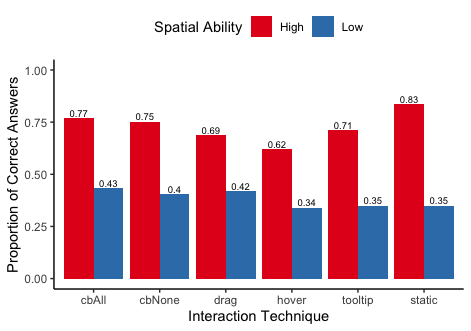
\includegraphics[width=\linewidth]{exp2_sa_by_interaction.png}
 \caption{Bar chart showing the proportion of participants answering the Bayesian reasoning task correctly by spatial ability and interaction technique. \remco{what's with the black lines above the bars? Is that a subtraction between the two bars? If so, remove please!}}
 \label{fig:exp2_sa_by_interaction}
\end{figure}

\subsubsection*{\textbf{Comparing Interaction Techniques within Spatial Ability Groups}}
Within each spatial ability group we performed a Chi-squared test of $accuracy \sim interaction\_technique$. Within the \textbf{high spatial ability} group we found a statistically significant difference in accuracy between participants using different interaction techniques ($\chi^2(5, N =  881) = 17.70, p < 0.01$). 

We performed pairwise Chi-squared tests with a Bonferroni corrected alpha ($0.003$) and found significant a pairwise difference between \textit{hover} and \textit{static} ($\chi^2(1, N = 287) = 13.60, p < 0.001$). The proportion of participants who were correct using \textit{hover} was $62\%$, whereas for the static visualization it was $83\%$ (Figure \ref{fig:exp2_sa_by_interaction}). 

Within the \textbf{low spatial ability} group we found no statistically significant difference in accuracy between participants using different interaction techniques ($\chi^2(5, N =  852) = 4.46, p = 0.49$). 

\remco{this is really cool! Would it make sense to take it one step further and look at (SA) x (interaction technique) x (base visualization)? The thought here is to see if the same message continues (that is to say, that good interactions need to be paired with good visualizations before it is useful.}
    
\subsection{Discussion} 
\remco{same comment as before... reorganize around hypotheses} Our analysis shows that interaction can narrow the performance gap between high and low spatial ability people in performing Bayesian reasoning (Figure \ref{fig:exp2_sa_by_interaction}). However it is important to note that this trend occurs in large part because \textbf{interaction decreases the performance of high spatial ability people compared to \textit{static}}. In some cases, such as with \textit{hover}, that decrease is statistically significant. On the other hand, our analyses indicate that overall \textbf{interaction increases the performance of low spatial ability people compared to \textit{static}} with the exception of \textit{hover} which produced lower accuracy than \textit{static} for both spatial ability groups.        


%\subsubsection*{H3.0}
%For every interaction technique, we found a statistically significant difference in $accuracy \sim high\_or\_low\_spatial\_ability$:
%\begin{itemize}
%	\item \textit{cbAll} ($\chi^2(1) = 25.74, p < 0.001$)
%	\item \textit{cbNone} ($\chi^2(1) = 48.23, p < 0.001$)
%	\item \textit{drag} ($\chi^2(1) = 23.14, p < 0.001$)
%	\item \textit{hover} ($\chi^2(1) = 33.94, p < 0.001$)
%	\item \textit{tooltip} ($\chi^2(1) = 52.42, p < 0.001$)
%	\item \textit{static} ($\chi^2(1) = 52.60, p < 0.001$)
%\end{itemize}

%Figure \ref{fig:accIntBaseSA} shows distributions of accuracy by each interaction technique and spatial ability and Table \ref{tab:accIntSA} shows the five number summaries plus mean and SD of accuracy for each interaction technique and spatial ability. 

%\subsubsection*{H3.1}
%Overall and within each base visualization and spatial ability group we performed  tests of $accuracy \sim interaction\_technique$. Results of each are presented below.  

%\subsubsection*{\textbf{Overall}}
%\textbf{High Spatial Ability}: Across all base visualizations we found a significant difference in accuracy between interaction techniques for people with high spatial ability ($\chi^2(5) = 21.12, p < 0.001$). A Dunn test with Bonferroni adjusted alpha showed the following significant pairwise differences:
%\begin{itemize}
%\item  \textit{cbAll} is significantly more accurate than \textit{hover} ($Z = 3.09, p-adj < 0.05$)
%\item  \textit{cbNone} is significantly more accurate than \textit{hover} ($Z = 3.09, p-adj < 0.05$)
%\item  \textit{hover} is significantly less accurate than \textit{static} ($Z = -4.02, p-adj < 0.001$)
%\end{itemize}
%Five number summaries plus mean and standard deviation are shown in Table \ref{tab:accIntSA} and Figure \ref{fig:accIntBaseSA}
 
%\noindent \textbf{Low Spatial Ability}: Across all base visualizations we found no significant difference in accuracy between interaction techniques for people with low spatial ability ($\chi^2(5) = 4.84, p = 0.44$). Five number summaries plus mean and standard deviation are shown in Table \ref{tab:accIntSA} and Figure \ref{fig:accIntBaseSA}.

%\begin{table}[h!]
%\resizebox{\linewidth}{!}{
%\centering
%\begin{tabular}{llllllll}
%  \hline
%  & Min & 1st Q & Median & 3rd Q & Max & Mean & SD \\ 
%  \hline
%cbAll - High SA & 0 & 100 & 100 & 100 & 100 & 89.5 & 21.5 \\ 
%  cbAll - Low SA & 0 & 12.5 & 62.5 & 100 & 100 & 60.3 & 41.3 \\ 
%  cbNone - High SA & 0 & 100 & 100 & 100 & 100 & 85.6 & 28.9 \\ 
%  cbNone - Low SA & 0 & 12.5 & 50 & 100 & 100 & 58.6 & 40.6 \\ 
%  drag - High SA & 0 & 75 & 100 & 100 & 100 & 81.8 & 31.1 \\ 
%  drag - Low SA & 0 & 0 & 75 & 100 & 100 & 58.9 & 42.5 \\ 
%  hover - High SA & 0 & 50 & 100 & 100 & 100 & 74.7 & 36.8 \\ 
%  hover - Low SA & 0 & 12.5 & 50 & 100 & 100 & 49.3 & 41.8 \\ 
%  tooltip - High SA & 0 & 75 & 100 & 100 & 100 & 84.2 & 28.7 \\ 
%  tooltip - Low SA & 0 & 12.5 & 50.9 & 100 & 100 & 57 & 40.3 \\ 
%  static - High SA & 0 & 100 & 100 & 100 & 100 & 90.3 & 24.6 \\ 
%  static - Low SA & 0 & 12.5 & 63.6 & 100 & 100 & 56.5 & 40.6 \\ 
 %  \hline
%\end{tabular}}
%\caption{Five number summary of accuracy for each interaction technique by high and low spatial ability (SA) across all base visualizations.  }
%\label{tab:accIntSA}
%\end{table}

%\subsubsection*{\textbf{Grouped}}
%\textbf{High Spatial Ability}: Within the grouped base visualization we found no significant difference in accuracy between interaction techniques for people with high spatial ability ($\chi^2(5) = 9.57, p = 0.09$). Five number summaries plus mean and standard deviation are shown in Table \ref{tab:accIntBaseSA} and Figure \ref{fig:accIntBaseSA}.

%\textbf{Low Spatial Ability}: Within the grouped base visualization we found no significant difference in accuracy between interaction techniques for people with low spatial ability ($\chi^2(5) = 1.69, p = 0.89$). Five number summaries plus mean and standard deviation are shown in Table \ref{tab:accIntBaseSA} and Figure \ref{fig:accIntBaseSA}.


%\subsubsection*{\textbf{Aligned}}
%\textbf{High Spatial Ability}: Within the aligned base visualization we found no significant difference in accuracy between interaction techniques for people with high spatial ability ($\chi^2(5) = 9.09, p = 0.11$). Five number summaries plus mean and standard deviation are shown in Table \ref{tab:accIntBaseSA} and Figure \ref{fig:accIntBaseSA}.

%\textbf{Low Spatial Ability}: Within the aligned base visualization we found no significant difference in accuracy between interaction techniques for people with low spatial ability ($\chi^2(5) = 8.74, p = 0.12$). Five number summaries plus mean and standard deviation are shown in Table \ref{tab:accIntBaseSA} and Figure \ref{fig:accIntBaseSA}.


%\subsubsection*{\textbf{Randomized}}
%\textbf{High Spatial Ability}: Within the randomized base visualization we found no significant difference in accuracy between interaction techniques for people with high spatial ability ($\chi^2(5) = 9.26, p = 0.10$). Five number summaries plus mean and standard deviation are shown in Table \ref{tab:accIntBaseSA} and Figure \ref{fig:accIntBaseSA}.

%\textbf{High Spatial Ability}: Within the randomized base visualization we found no significant difference in accuracy between interaction techniques for people with low spatial ability ($\chi^2(5) = 1.76, p = 0.88$). Five number summaries plus mean and standard deviation are shown in Table \ref{tab:accIntBaseSA} and Figure \ref{fig:accIntBaseSA}.

%\begin{table}[h!]
%\resizebox{\linewidth}{!}{
%\centering
%\begin{tabular}{llllllll}
%  \hline
%  & Min & 1st Q & Median & 3rd Q & Max & Mean & SD \\ 
%  \hline
%grouped - cbAll - High SA & 12.5 & 100 & 100 & 100 & 100 & 91.5 & 21.9 \\ 
%  grouped - cbAll - Low SA & 0 & 12.5 & 100 & 100 & 100 & 66.2 & 43.9 \\ 
%  grouped - cbNone - High SA & 0 & 100 & 100 & 100 & 100 & 85.8 & 28.8 \\ 
%  grouped - cbNone - Low SA & 0 & 12.5 & 62.5 & 100 & 100 & 58.8 & 42.3 \\ 
%  grouped - drag - High SA & 12.5 & 100 & 100 & 100 & 100 & 89.4 & 22 \\ 
%  grouped - drag - Low SA & 0 & 0 & 75 & 100 & 100 & 56.2 & 45.2 \\ 
%  grouped - hover - High SA & 0 & 50 & 100 & 100 & 100 & 73.7 & 37.4 \\ 
%  grouped - hover - Low SA & 0 & 0 & 50 & 100 & 100 & 53 & 44.8 \\ 
%  grouped - tooltip - High SA & 0 & 93.2 & 100 & 100 & 100 & 85.5 & 28.3 \\ 
%  grouped - tooltip - Low SA & 0 & 12.5 & 50 & 100 & 100 & 56.9 & 40.4 \\ 
%  grouped - static - High SA & 0 & 100 & 100 & 100 & 100 & 90.2 & 25.4 \\ 
%  grouped - static - Low SA & 0 & 6.3 & 75 & 100 & 100 & 56.4 & 42.3 \\ 
%  aligned - cbAll - High SA & 50 & 100 & 100 & 100 & 100 & 92.6 & 16.7 \\ 
%  aligned - cbAll - Low SA & 0 & 25 & 75 & 100 & 100 & 61.8 & 41.7 \\ 
%  aligned - cbNone - High SA & 0 & 100 & 100 & 100 & 100 & 88.5 & 24.7 \\ 
%  aligned - cbNone - Low SA & 0 & 50 & 100 & 100 & 100 & 68.6 & 37.9 \\ 
%  aligned - drag - High SA & 0 & 50 & 100 & 100 & 100 & 73.8 & 38.1 \\ 
%  aligned - drag - Low SA & 0 & 9.4 & 75 & 100 & 100 & 59.8 & 41.3 \\ 
 % aligned - hover - High SA & 0 & 75 & 100 & 100 & 100 & 80.2 & 33.6 \\ 
 % aligned - hover - Low SA & 0 & 0 & 50 & 100 & 100 & 45.1 & 40.7 \\ 
 % aligned - tooltip - High SA & 0 & 75 & 100 & 100 & 100 & 83.5 & 29.4 \\ 
%  aligned - tooltip - Low SA & 0 & 12.5 & 51.7 & 100 & 100 & 59.2 & 39.8 \\ 
%  aligned - static - High SA & 12.5 & 100 & 100 & 100 & 100 & 92.8 & 20.1 \\ 
%  aligned - static - Low SA & 0 & 40.6 & 75 & 100 & 100 & 61.3 & 39.3 \\ 
%  randomized - cbAll - High SA & 0 & 75 & 100 & 100 & 100 & 86.2 & 24 \\ 
%  randomized - cbAll - Low SA & 0 & 9.4 & 50 & 100 & 100 & 54.2 & 39.9 \\ 
%  randomized - cbNone - High SA & 0 & 75 & 100 & 100 & 100 & 82.2 & 33.1 \\ 
%  randomized - cbNone - Low SA & 0 & 12.5 & 50 & 100 & 100 & 49.6 & 39.6 \\ 
%  randomized - drag - High SA & 0 & 66.5 & 100 & 100 & 100 & 82.6 & 29.8 \\ 
%  randomized - drag - Low SA & 0 & 12.5 & 50 & 100 & 100 & 60.4 & 42.2 \\ 
%  randomized - hover - High SA & 0 & 50 & 100 & 100 & 100 & 71 & 38.7 \\ 
%  randomized - hover - Low SA & 0 & 12.5 & 50 & 100 & 100 & 49.8 & 40.6 \\ 
 % randomized - tooltip - High SA & 0 & 75 & 100 & 100 & 100 & 83.8 & 28.8 \\ 
 % randomized - tooltip - Low SA & 0 & 0 & 62.5 & 100 & 100 & 54.3 & 41.4 \\ 
%  randomized - static - High SA & 0 & 100 & 100 & 100 & 100 & 88.8 & 27 \\ 
 % randomized - static - Low SA & 0 & 3.1 & 50 & 98.7 & 100 & 49.8 & 40 \\ 
 %  \hline
%\end{tabular}}
%\caption{Five number summary of accuracy for each interaction technique by high and low spatial ability (SA) and base visualizations. }
%\label{tab:accIntBaseSA}
%\end{table}

%\begin{figure}[h!]
%\centering
%\begin{tabular}{ll}
%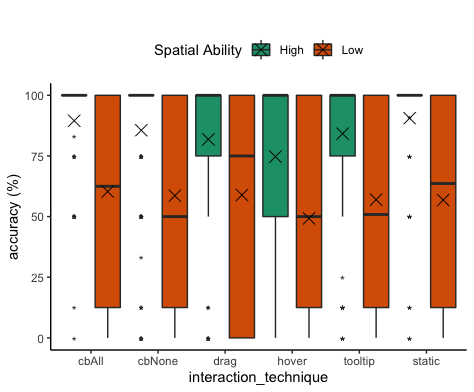
\includegraphics[height=100px]{accIntSA.png} & 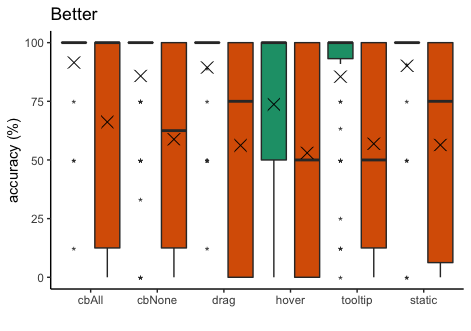
\includegraphics[height=85px]{accIntSAGrouped.png}  \\   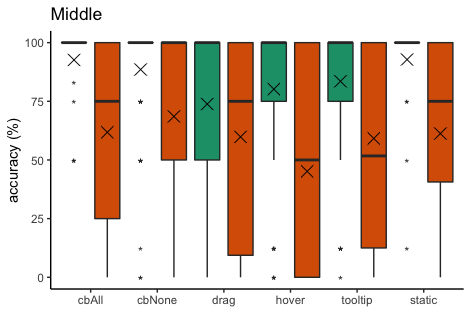
\includegraphics[height=85px]{accIntSAAligned.png} & 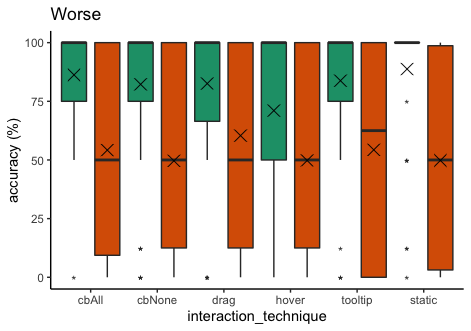
\includegraphics[height=85px]{accIntSARandomized.png} 
%\end{tabular}
% \caption{Boxplots showing the distributions of $accuracy \sim interaction\_technique * spatial\_ability$ overall (top left) and for each base visualization. X represents the mean of each distribution.}
% \label{fig:accIntBaseSA}
%\end{figure}

%\subsection{Discussion}
%Our analyses indicate that we should accept \textbf{H3.0} (there will be a significant difference in accuracy between high and low spatial ability participants for every interaction technique). No interaction techniques removed the significant difference in performance between high and low spatial ability participants.  

%Our analyses also indicate that we should accept \textbf{H3.1} (the effect of different interaction techniques on accuracy will differ between participants with high versus low spatial ability). However, not in the way we expected. Ultimately, our analyses indicated that low spatial ability participants are not significantly affected by any interaction techniques; their performance is low across the board. In contrast, we find that overall base visualizations the accuracy of high spatial ability participants could be significantly decreased by certain interaction techniques. Specifically, \textit{hover} which we found to be significantly less accurate than \textit{cbAll}, \textit{cbNone}, and even \textit{static} for high spatial ability participants.  


